\subsection{Multi-source multi-view network estimation}
\label{sec:vis2net}

The approach presented in Section \ref{sec:activity} provides multiple types of visual cues that are socially informative, especially social interactions. In this section, we propose the paradigm by which we sense the network from these heterogenous visual cues. To this end, we begin with an undirected weighted graph $G$ of $K$ nodes, with a non-negative weight associated with each edge between a pair of nodes, to represent a community of $K$ members, where the weight depicts the closeness, or ties, between the two member. However as we have argued and has been found in the conventional social network analysis, a social network is in multiple views, and a more appropriate representation should account for the realistic conditions arising from multiple sources of visual cues. 

First, to represent a network in $V$ views, we define $G\triangleq\{A^{(v)}\}$, where the matrix $A^{(v)}, v=1,2,\cdots,V$ is a symmetric affinity matrix describing the closeness or ties between every pair of two members in the $v$th view. Meanwhile, assume that there exist $S$ types of low-level `sensors' which provide $S$ types of socially informative cues $\vy^s, s=1,2,\cdots,S$, where $\vy^s(i,j)$ denotes the description about the pairwise or relative visual cues between human $i$ and human $j$, and these visual cues are relevant to the network of $V$ views $A^{(v)}, v=1,2,\cdots,V$.  As an example, suppose that we have successfully detected and tracked two faces $i$ and $j$, and through the state-of-art computer vision techniques we have computed a set of five descriptors characterizing five types of visual cues, including: 1) Relative positions of the two detections (denoted as $\vy^1$, where $\vy^1(i,j)$ denotes the relative poses between human $i$ and human $j$. The same notion applies for the remaining visual cues.); 2) relative gazes (denoted as $\vy^2$); 3) relative body poses (denoted as $\vy^3$); 4) their participation in social interactions as detected from Section \ref{sec:activity} (denoted as $\vy^4$); and 5) scene classification (denoted as $\vy^5$).

If a view refers to a specific type of visual feature or low-level cue computed by a particular computer vision algorithm, where for example the social relationship between two humans can be described in two views - the frequency they participate in a social interaction, and the number of their co-occurrence in pictures, then we may directly reach two affinity matrices $A^{(1)}$ and $A^{(2)}$, then the affinity weight comes directly or via simple heuristic derivation from the visual features, e.g., from $\vy^4$.  However, this may not be true for the common case that the views correspond to higher-level semantics such as the different types of roles or memberships\cite{AiroldiBFX08,Kim12} that are not directly or explicitly related to the low-level visual cues, and in particular when the available types of low-level visual cues are much more than the number of views of interest.  Moreover, these high-level views usually embeds overlapping community structures, meaning that the members belongs to different clusters in each view, within each of which the members share close ties with each other, and members from different clusters are different from each other. 

To explain, consider that the network we expect to estimate is a three-view network, where $A^{(1)}, A^{(2)}, A^{(3)}$ all take values in $[0,1]$ indicating the probabilities of the two individuals belonging to the specific types of relationship: friend, family, and workmates. At their extreme values, $A^{(1)}(i,j)=1$ means the two people are friends and $A^{(1)}(i,j)=0$ means that they do not get along with each other well,  $A^{(2)}(i,j)=1$ means the two people definitely belong to the same family and $A^{(2)}(i,j)=0$ means otherwise, and $A^{(3)}(i,j)=1$ means the two people are workmates and $A^{(2)}(i,j)=0$ means otherwise. For a group of members who are mutually each others family members, workmates, or friends, the clustering patterns for the families, for the career, and for friendship are all different, while each member can be fully situated in each and every of these types of communities. In this example, it is unclear how we may derive the binary socially-characteristic quantities $A$'s from the low-level visual cues $\vy^1$ to $\vy^5$, and existing social network research has not provided us a solution to our knowledge.

We seek an unified learning-based paradigm to obtain the multi-view network representations (affinity matrices) from the multiple low-level heterogeneous visual cues. We refer to this architecture as multi-source multi-view network estimation. Our architecture consists of $V$ `oracles' $\Psi_{v}$ that we aim to learn, each of which is an estimator $\hat{A}^{(v)}$ of view $v$ from descriptor $\bar{\vy}=[\vy^1,\vy^2, \cdots,\vy^S$, i.e., $\hat{A}^{(v)}=\Psi_{v}(\bar{\vy})$. Assume that we have $N$ samples of graphs for which we have computed their visual cues $\{\bar{\vy}_{n}\}_{n=1,2,\cdots,N}$  from related imagery. Meanwhile, there may (or may not) be another small collection of $M(<<N)$ sample graphs for which we have computed their visual cues $\{\bar{\vy}_{m}\}_{m=1,2,\cdots,M}$ and had their `ground-truth' affinities $\{\bar{A}^{(v)}_{m}\}_{m=1,2,\cdots,M}$ (These ground-truths are available, for instance, through our prototype system as to be introduced in Section \ref{sec:sys}). Then, the overall learning objective can be represented as 
\begin{equation}\label{eq:sensing}
\{\Psi^{*}_{v}\}=\arg\min_{\{\Psi_{v}\},\{\hat{A}^{(v)}_l\}_{l=1}^{N+M}}\sum_{m=1}^{M}\mathcal{J}(\{\Psi_{v}\}, \{\bar{\vy}_m\}, \{\bar{A}^{(v)}_m\})+\sum_{l=1}^{N+M}\tau(\{\hat{A}^{(v)}_l\})+\gamma(\{\Psi_{v}\}).
 \end{equation}
 
Specifically, we use the first term $\mathcal{J}$ to enforce the estimation quality of the oracles on supervised samples, for example, by defining
\begin{equation}\label{eq:L2error}
\mathcal{J}(\{\Psi_{v}\}, \{\bar{\vy}_m\}, \{\bar{A}^{(v)}_m\})=\sum_{v=1}^{V}\|\Psi_{v}(\vy_m)-A^{(v)}_m\|^{2},
 \end{equation}
such that the estimated network is as close as possible to the `ground-truth' in the sense of minimal $l_2$ error between the affinity matrices. One may imagine that a least square regression suffices, and other powerful regression machines exist, such as Gaussian process regression \cite{GPbook} or deep learning \cite{DLbook}. However, socially-compatible estimations requires more than conventional estimations, in the sense that the individual oracles must give compatible estimates across views. Two nodes inferred as family members by one oracle, for example, should receive low confidence score from the friendship oracle which claims that they are adversary to each other. We use the penalty $\gamma$ to enforce the compatibility among oracles. Finally, we have been fully aware of the community clustering effects of real-world social networks, and therefore we incorporate penalty $\tau$ as well to enforce the clustering effect within the estimated affinity matrix, so that if node $i$ and node $j$ are both inferred as family members of node $k$ we will have the same inference for the relationship between $i$ and $j$. We will explore optimal formats for $\gamma$ and $\tau$ by, e.g., employing or extending the common used network priors summarized in \cite{Goldenberg}. Cross-view compatibility and within-view clustering are essential to our multi-source estimation from low-level visual cues, and this socially-aware sensing architecture, dissimilar to any other regression machines which take in and output independent samples, is at the heart of our proposed socially-aware visual sensing paradigm.


%\begin{figure}[t!]
%\begin{center}
%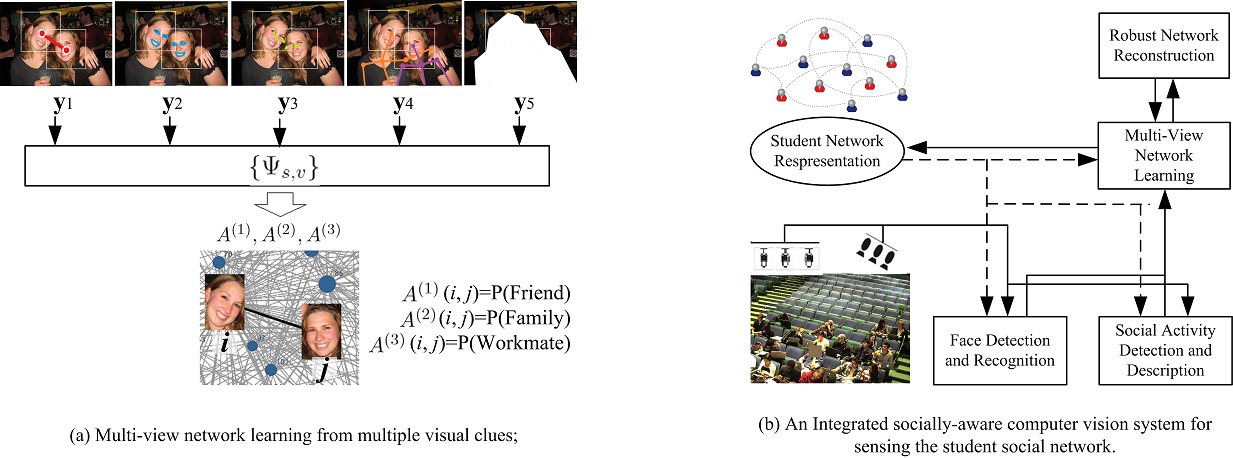
\includegraphics[width=\columnwidth]{featurelearn}
%\end{center}
%\vspace{-0.25in} \caption{\captionsize 
%Illustrations for the problem of multi-view network learning from multiple low-level visual clues and the framework of integrated socially-aware computer vision for understanding student netwrok. \label{fig:featurelearn}\afterfigspace}
%\end{figure}






%%%%%%%%%%%%%%%%%%%%%%%%%%%%%%%%%%%%%%%%%%%%%%%%%%%%%%%%%

\subsubsection{Associating identities with image targets}
\label{sec:assoc}

To obtain the low-level visual descriptions $\vy^s$ between individual $i$ and individual $j$, we must first identify the two individuals from the detections in images or tracks in videos. While the state-of-art face recognizer has achieved compellingly outstanding performance even for the faces `in the wild', there always remain ambiguities and errors. Suppose that from an image we have detected $L$ faces or from a video we have tracked $L$ faces, and that the face recognizer outputs a $K$-dimensional probabilistic histogram $h_l$ for the $l$th target in the image or video, with $h_m(k)$ describing the likelihood for this target to belong to the $k$th identity. We must assign each of these $L$ targets to one of the possible $K$ identities of interest for the social network estimation approach to work. 

The problem of uncertainties in node identities is uncommon for conventional social network research, where the nodes are mostly straightforwardly identifiable. However, the problem is unique and crucial for network sensing from image data, because of the nodes in the network are indirectly related to image targets via a face/human detector and/or a visual tracker, especially when we aim to accumulate social evidences from many image/video samples.

We propose to explore robust algorithms that may properly handle the non-robustness of a face recognizer and provide identity assignments that are less sensitive to the erroneous output from a face recognizer. A preliminary solution can be straightforward as follows. Instead of assigning each target to a single identity from $K$ possible ones that might be incorrect, consider that To leverage and properly aggregate these likelihood conveyed from face recognition, we may first enumerate all $\prod_{l=0}^{L-1}(K-l)$ possible assignments. We then may duplicate the original image or video into $\prod_{l=0}^{L-1}(K-l)$ copies, in each of which we may assume that the $L$ targets have a determined identity assignment $\{k_1, k_2, \cdots, k_L\}, k_l\in\{1,2, \cdots, K\}$. We allow all these $\prod_{l=0}^{L-1}(K-l)$ `hallucinated' samples to be used for computing low-level description $\vy^s$, where the $(i,j)$-pair of targets will contribute to the descriptor $\vy^s(k_i,k_j)$, with appropriate pooling strategy to effective and efficiently aggregate all contributions from the expanded set of $\prod_{l=0}^{L-1}(K-l)$ new samples. A `maximum-pooling' approach, for example, may be employed by determining $k_l^{*}=\max_{k}h_l(k)$, the most probable identity for target $l$, and use the only maximum assignment $\{k_1^{*}, k_2^{*}, \cdots, k_L^{*}\}$ to compute the visual cues between individuals specified by $\{k_1^{*}, k_2^{*}, \cdots, k_L^{*}\}$. This strategy is essentially identical to the idea of assigning each target to a single (possibly incorrect) identity. Alternatively, we may adopt a weighted average pooling, where the hallucinated image/video with assignment $\{k_1, k_2, \cdots, k_L\}$ will contribute to the visual cues but with a confidence score, for example, of $\prod_{l=1}^{L}h_l(k_l)$.

We propose to develop and evaluate other systematic solutions during the award period. We foresee that our treatment to this problem may lead to new results in decision theory and statistical signal processing on graphs and other kinds of relational data.

